
Although many RDF triple stores have been proposed during the past
few years, most of them were designed and optimized mainly for
non-spatial Semantic Web data. In order to enable spatial query
processing on RDF triple stores, the state-of-the-art
method~\cite{conf/gis/BrodtNM10} is to treat all the Universal
Resource Identifiers (URIs) and literals, non-spatial or spatial,
equally and replace each URI and literal with an integer ID by
dictionary encoding. As a result, each spatial literal (e.g., the
latitude and longitude coordinates or the address) is mapped to a
randomly generated ID. Afterwards, an R-tree (or its
variant)~\cite{reference/gis/HadjieleftheriouMTT08} is created to
index all the IDs referred to spatial literals. However, this
dictionary encoding-based method may incur extreme inefficiency in
evaluating spatial queries on RDF triple stores, especially when
coping with large-scale spatial data
sets~\cite{conf/gis/BrodtNM10}. In this article, we employ a novel
representation, \emph{GeoHilbert} -- an RDF vocabulary as an
extension of the Geography Markup Language (GML), to model spatial
features based on their Hilbert
curve~\cite{journals/tkde/MoonJFS01} transformation information
and to utilize Spatially Aware Mapping (SAM), instead of
dictionary mapping, to encode URIs and literals for preserving
spatial locality.


\subsection{Data Representation}

Because many huge data repositories published online contain
geographic location or spatial relationship information, we are
witnessing a new research trend of modeling geographic entities
ontologically and querying their spatial relations in the Semantic
Web community. As one of the Semantic Web technologies, the
Resource Description Framework treats relationships as first-class
citizens and, consequently, can work as an ideal tool for modeling
and querying complex and large amounts of relations between
spatial entities. The XML formatted semantic data can be converted
to the corresponding RDF representation with minor modifications.
For example, Listing~\ref{list2} shows an XML data excerpt from
the OpenStreetMap project\footnote{http://www.openstreetmap.org/}.
This snippet describes the referred information (semantic and
spatial) about a restaurant in Pasadena, California, USA. Its
corresponding RDF representation is demonstrated in
Listing~\ref{list3}. Specifically, \emph{gml} represents the
namespace\footnote{http://www.opengis.net/gml} of the GML
standard, and \emph{gstore} corresponds to the
namespace\footnote{http://example.org/gstore} of our Geo-Store
system.

%The RDF data is a collection of RDF triples, and each RDF triple
%is of the form $\langle subject, predicate, object \rangle$, where
%\emph{subject} is the URI of a resource, \emph{predicate}
%represents a particular relationship, and \emph{object} denotes a
%URI of another resource or a literal.

%Table~\ref{tab-prefix} shows the namespace prefixes used in this
%article.

\lstset{showstringspaces=false} \lstset{basicstyle=\ttfamily\small,escapeinside={`}{`}}

\begin{lstlisting}[caption={An XML data excerpt from the OpenStreetMap project.},
                  language=SQL,
                  label={list2},
				  frame=single]
- <node id="738330640" lat="34.1135498" lon="-118.1235345" user="AM909" uid="82317"
 visible="true" version="1" changeset="4737707"  timestamp="2010-05-18T11:26:40Z">
  <tag k="amenity" v="restaurant" />
  <tag k="cuisine" v="american" />
  <tag k="name" v="Colonial Kitchen" />
  <tag k="source" v="usgs_imagery;survey;image" />
  <tag k="source_ref" v="AM909_DSCU3253" />
  </node>
\end{lstlisting}


\lstset{showstringspaces=false} \lstset{basicstyle=\ttfamily\small,escapeinside={`}{`}}

\begin{lstlisting}[caption={The RDF representation of the restaurant described in Listing~\ref{list2}.},
                  language=SQL,
                   label={list3},
                   frame=single]
...
gstore:Point738330640   gml:amenity     "restaurant"
gstore:Point738330640   gml:cuisine     "american"
gstore:Point738330640   gml:name        "Colonial Kitchen"
gstore:Point738330640   gml:pos         "34.1135498  -118.1235345"
...
\end{lstlisting}

%\begin{table}[!h]
%\small{
%\begin{center}
%\vspace*{-0pt}
%\begin{tabular}{|p{1.5in}|p{2.0in}|}
%\hline \textbf{Namespace Prefix} & \textbf{URI} \\ \hline \hline
%gml & http://www.opengis.net/gml  \\
%\hline
%gstore & http://example.org/gstore \\
%\hline
%\end{tabular}
%\end{center}
%\vspace*{-10pt} \caption{Namespace prefixes used in this article.}
%\label{tab-prefix} }
%\end{table}

\subsection{System Architecture}

Figure~\ref{fig-framework} shows the system framework of the
Geo-Store system, which consists of four main components: query
parser and planner module, spatially aware mapping module,
internal processing module, and dictionary decoding module.

\begin{figure*}[!h]
\begin{center}
%\hspace*{30pt}
\centerline{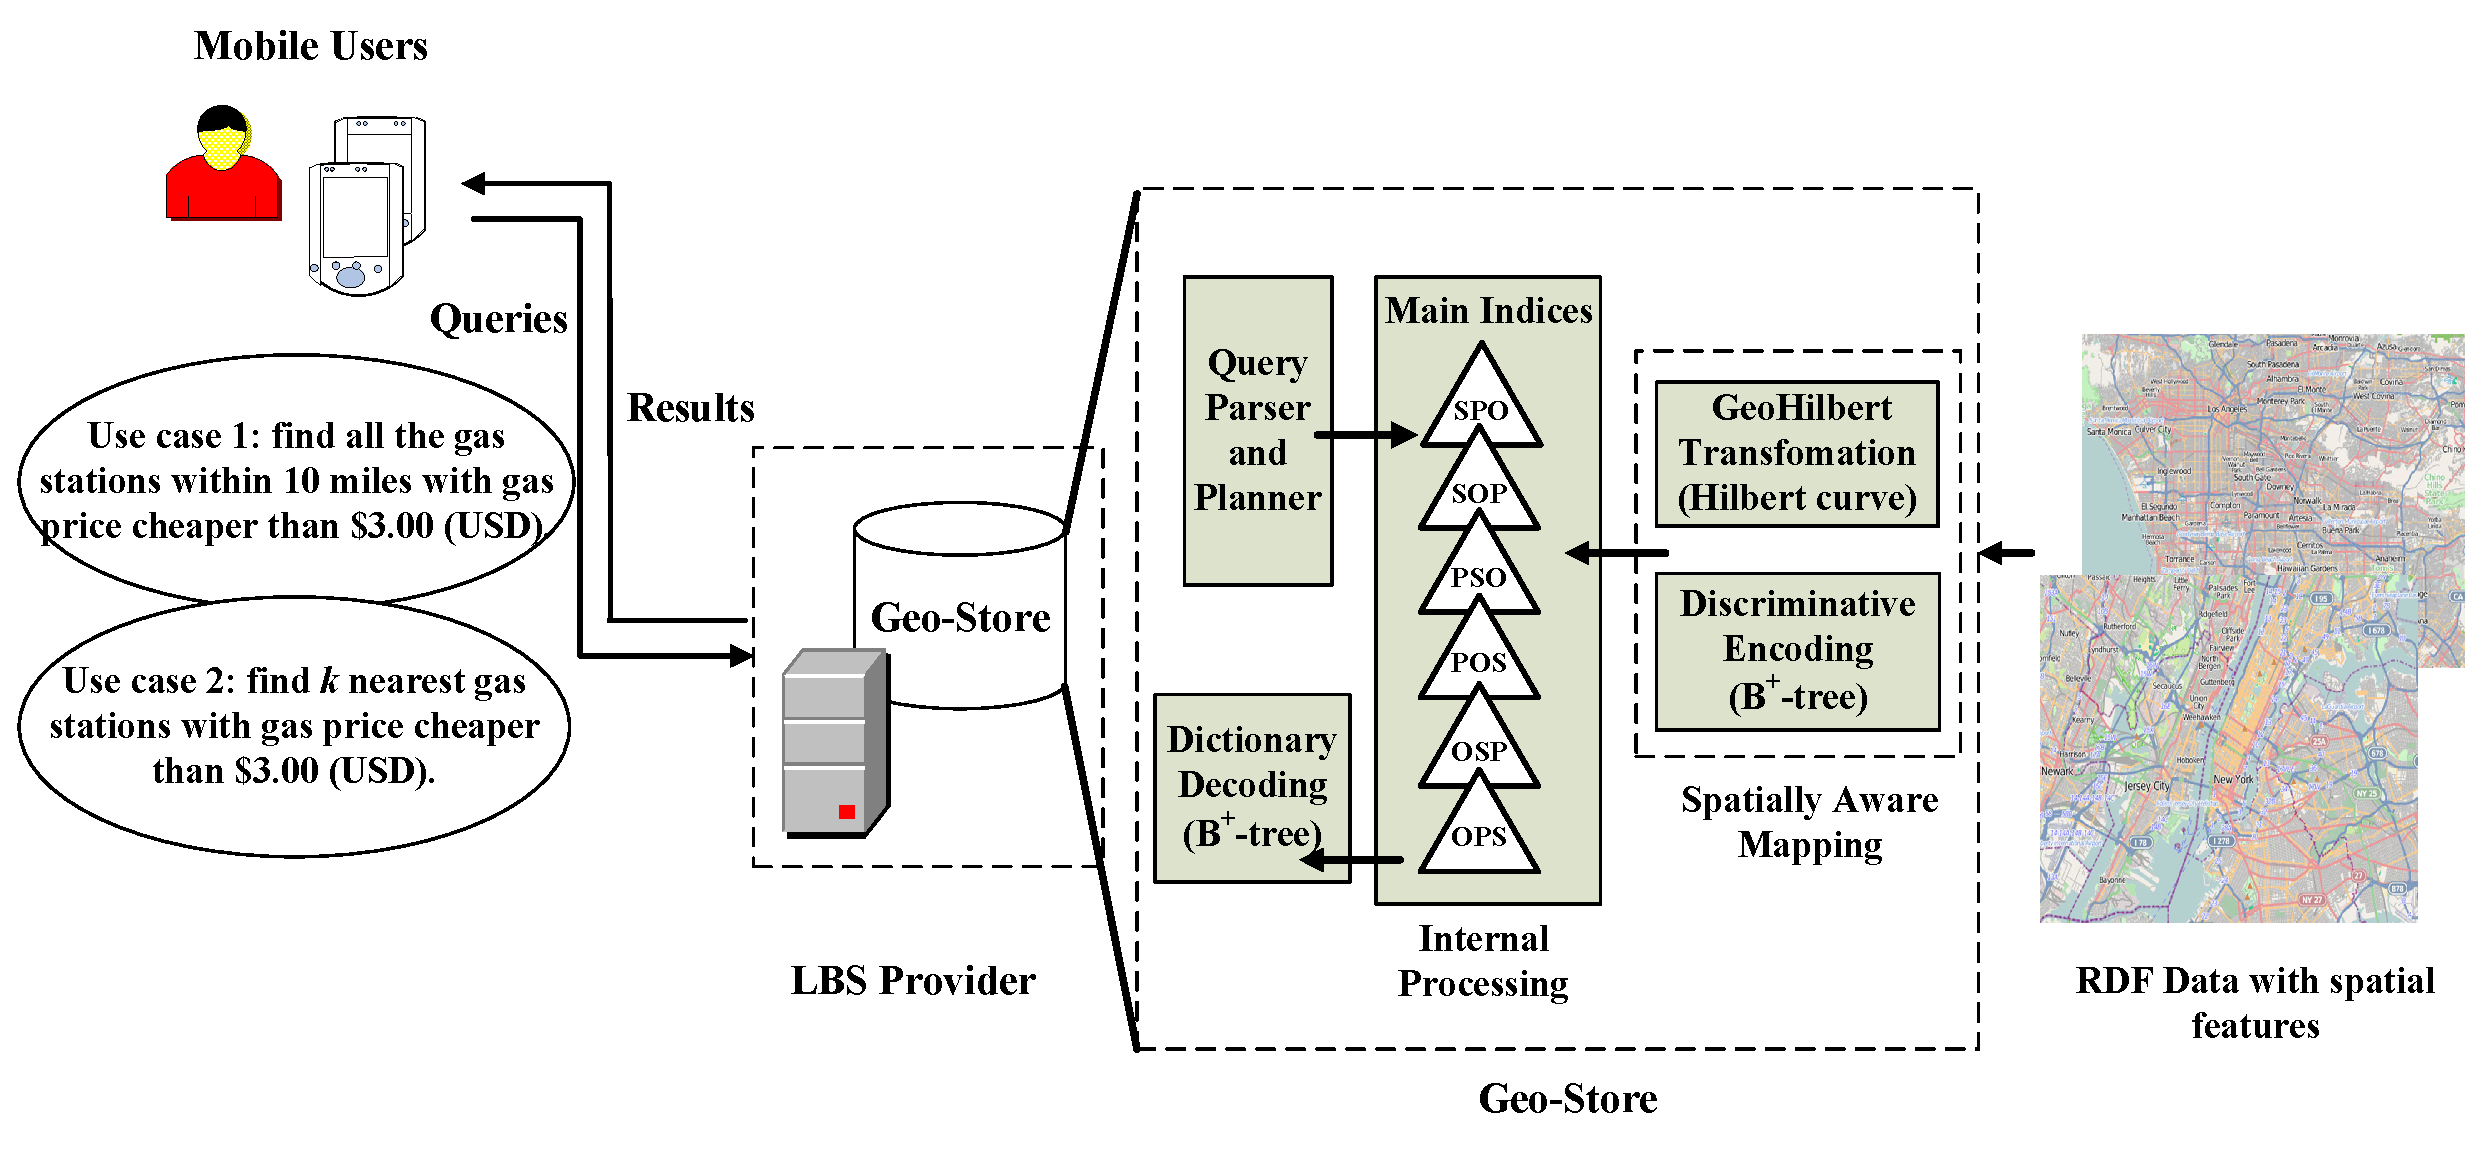
\psfig{file=geo-store-journal/image/framework2.eps,width=6.5in}}
\caption{Geo-Store system architecture and use cases.}
\label{fig-framework} \vspace*{-10pt}
\end{center}
\end{figure*}


\subsubsection{Spatially Aware Mapping Module}

In most of the existing triple stores, each URI or literal is
replaced with a unique integer ID by dictionary mapping because
the triples may contain very long URIs and string literals. In our
system, in order to support efficient spatial query evaluation on
triples, we extend the standard dictionary encoding and design a
Spatially Aware Mapping (SAM) approach to encode all the URIs and
literals, as well as preserve spatial locality. SAM includes two
major components, \emph{GeoHilbert Transformation} and
\emph{Discriminative Encoding}. With GeoHilbert Transformation,
original RDF triples are transformed to the corresponding
GeoHilbert representation. In addition, SAM assigns an ID to each
URI and literal in a discriminative way in order to maintain
spatial locality by executing the discriminative encoding
component.


\paragraph{GeoHilbert Transformation}

We utilize a novel RDF representation, GeoHilbert, to model
spatial data in Geo-Store. GeoHilbert is designed for
incorporating the Hilbert curve-based spatial transformation
information into original RDF data. GeoHilbert consists of a
subject, \emph{HilbertMapping} and four predicates:
\emph{StartPoint}, \emph{Order}, \emph{Orientation}, and
\emph{Pos}. Specifically, the values of \emph{StartPoint},
\emph{Order}, \emph{Orientation}, and \emph{Pos} are the location
of the Hilbert curve starting point, the curve order $O$, the
curve orientation $\theta$, and a Hilbert value translated from a
given spatial location, respectively.

Listing~\ref{list4} demonstrates the corresponding RDF data in the
GeoHilbert representation for the restaurant described in
Listing~\ref{list2}. As shown in Listings~\ref{list3}
and~\ref{list4}, the GeoHilbert representation appends to the
original RDF representation an additional RDF statement,
\{\emph{gstore:Point738330640}, \emph{gstore:Pos},
\emph{``208083"}\}, which stores the relative position of the
referred point along the Hilbert space-filling curve.

%\newpage

\begin{lstlisting}[caption={The GeoHilbert representation of the restaurant described in Listing~\ref{list2}.},
                  %language=SQL,
                   label={list4},
                   frame=single]
...
gstore:HilbertMapping  gstore:StartPoint   "32.3372200  -114.1369000"
gstore:HilbertMapping  gstore:Order        "10"
gstore:HilbertMapping  gstore:Orientation  "Up Left"
...
...
gstore:Point738330640   gml:amenity     "restaurant"
gstore:Point738330640   gml:cuisine     "american"
gstore:Point738330640   gml:name        "Colonial Kitchen"
gstore:Point738330640   gml:pos         "34.1135498  -118.1235345"
gstore:Point738330640   gstore:Pos      "208083"
...
\end{lstlisting}


\paragraph{Discriminative Encoding}

The Discriminative Encoding (DE) component takes the GeoHilbert
representation based data as the input. For each literal following
the predicate \emph{Pos}, DE assigns it a positive ID which is
exactly the same as its Hilbert value. For example, in
Listing~\ref{list4}, the literal \emph{``208083"} in the triple
\{\emph{gstore:Point738330640}, \emph{gstore:Pos},
\emph{``208083"}\} will be assigned with ID \emph{208083}. For all
the other literals or URIs, DE acquires a random integer by
calling a dictionary encoding function, and then returns the
opposite of that integer as the ID (e.g., a randomly generated
integer ``1000" will be returned as ``$-$1000"). All the assigned
IDs are maintained in a B$^{+}$-tree to speed up the dictionary
lookup.


\subsubsection{Internal Processing Module}

Generally, the evaluation of SPARQL queries is based on pattern
matching. In this system, we maintain in memory all six possible
permutations of \emph{subject} (S), \emph{predicate} (P), and
\emph{object} (O) in six separate indices in order to guarantee
that every possible query pattern in a SPARQL query with variables
in any position of a triple can be answered by only performing a
single index scan. Specifically, these permutations are named as
SPO, SOP, OSP, OPS, PSO, and POS indices, respectively. Notice
that instead of the original URIs or literals, all the six indices
here consist of integer IDs, which are assigned by the
discriminative encoding component. This ID-based indexing scheme
can both save memory space and accelerate join processing.


\subsubsection{Query Parser and Planner Module}

When Geo-Store receives a SPARQL query $q$, it parses $q$,
identifies the IDs that have been assigned to the literals in $q$
according to SAM, and employs the retrieved IDs to replace the
corresponding literals in $q$. By executing these processes, the
subsequent evaluation of $q$ purely relies on the comparisons of
IDs instead of the original literals. A query evaluation plan can
then be generated accordingly.


\subsubsection{Dictionary Decoding Module}

After the SPARQL query is evaluated by the internal processing
module, the dictionary decoding module transforms the resulting
IDs back to their original literals as the query results. In
Geo-Store, we employ a B$^{+}$-tree structure to implement this
ID-to-literal mapping.
